\documentclass[11pt]{article}
\usepackage{csc766}

%%%%%%%%%%%%%%%%%%%% name/id
\rfoot{\small Brian Park | 200190057}


%%%%%%%%%%%%%%%%%%%% Course/HW info
\newcommand*{\instr}{Xipeng Shen}
\newcommand*{\term}{Spring 2023}
\newcommand*{\coursenum}{CSC 766}
\newcommand*{\coursename}{Code Optimization for Scalar and Parallel Programs}
\newcommand*{\hwnum}{2}

\rhead{\LARGE   \fontfamily{lmdh}\selectfont	HW \hwnum}

\lfoot{\small \coursenum, \term, HW \hwnum}

%%%%%%%%%%%%%%%%%%%%%%%%%%%%%% Document Start %%%%%%%%%%%%%%%%%
\begin{document}

%%%%%%%%%%%%%%%%%%%%%%%%%%%%%%%%%%%%%%%%%%%%%%%%%%%%%%%%%%%%%%%%%%%%%%%%%%%%%%%%%%%%%%%%
% Question 1
%%%%%%%%%%%%%%%%%%%%%%%%%%%%%%%%%%%%%%%%%%%%%%%%%%%%%%%%%%%%%%%%%%%%%%%%%%%%%%%%%%%%%%%%
\section{}

Convert the following loop to a form where the loop indexes are each incremented by 1:
\begin{verbatim}
for(i=50;i>=10;i=i-7) 
    X[i,i+1]=0;
\end{verbatim}

\begin{Answer}
\begin{verbatim}
for(i=0;i<=5;i=i+1) 
    X[i*7+15,i*7+16]=0;
\end{verbatim}
\end{Answer}
\newpage
\section{}
\begin{enumerate}[a)]
\item
\begin{verbatim}
for (i=1; i<30; i++)
    for (j=i+2; j<40-i; j++)
        X[i,j]=0;
\end{verbatim}

\item
\begin{verbatim}
for (i=10; i<=1000;i++) 
    for (j=i; j<i+10; j++)
        X[i,j]=0;
\end{verbatim}

\item
\begin{verbatim}
for (i=1; i<100; i++)
    for (j=0; j<100+i; j++)
        for (k=i+j; k<100-i-j; k++) 
            X[i,j,k]=0;
\end{verbatim}

\end{enumerate}
\begin{enumerate}
	\item Draw the iteration spaces for (a) and (b).
		\begin{Answer}
		\begin{figure}[H]
		    \centerline{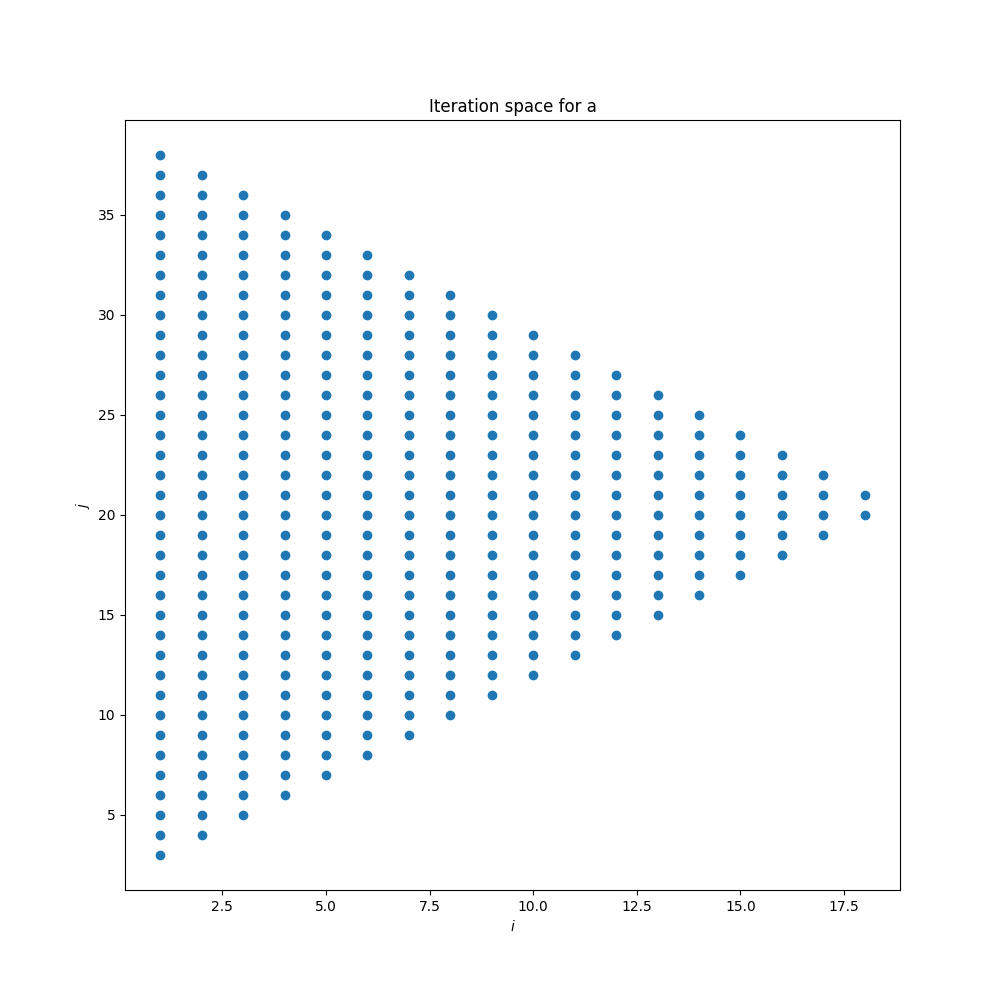
\includegraphics[width=6in]{figures/iteration_space_a.png}}
		\end{figure}
		\begin{figure}[H]
		    \centerline{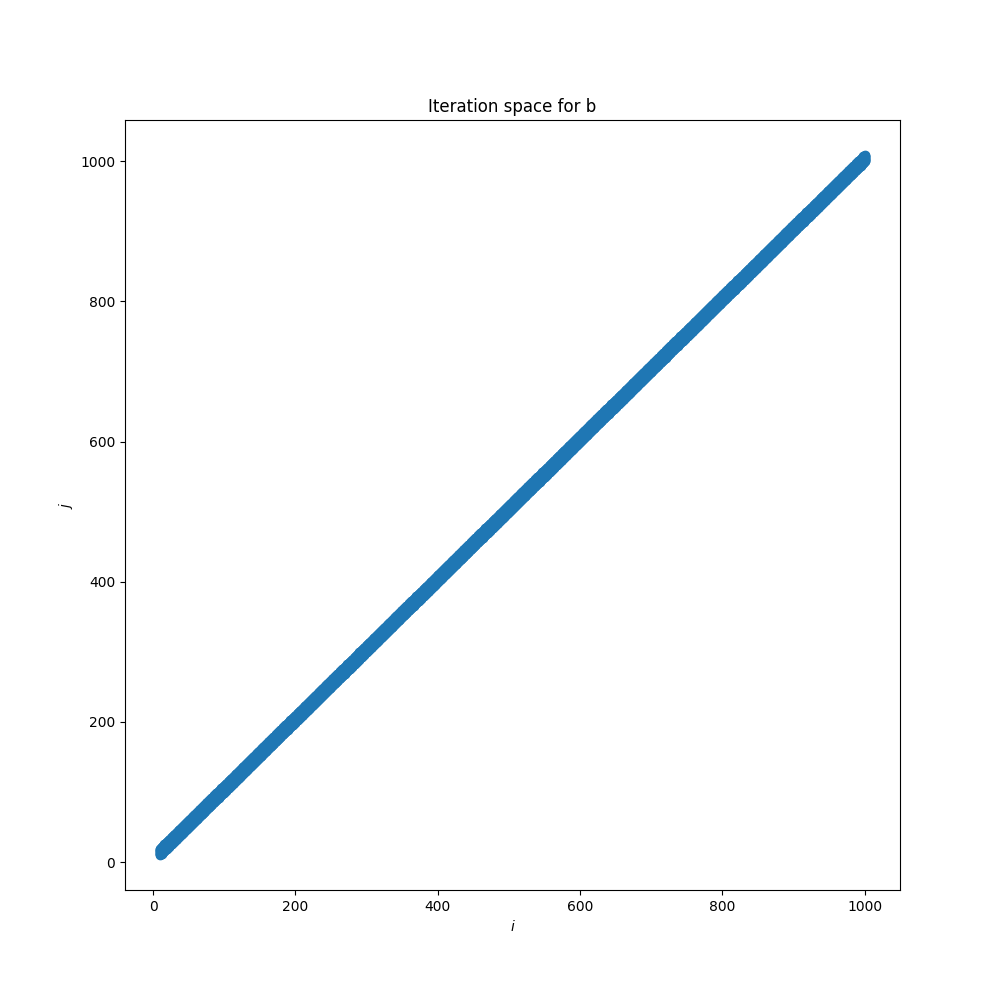
\includegraphics[width=6in]{figures/iteration_space_b.png}}
		\end{figure}
		\end{Answer}
		\newpage
	\item Write the constraints in matrix form (i.e., give the values of the vectors $i$ and $b$ and the matrix $B$.)
		\begin{Answer}
		a.
		$$
		\begin{pmatrix}
		1 & 0  \\
		-1 & 0  \\
		-1 & 1 \\
		-1 & -1 \\
		\end{pmatrix}
		\begin{pmatrix}
		i \\
		j 
		\end{pmatrix}
		+
		\begin{pmatrix}
		-1 \\
		-29 \\
		-2 \\
		39
		\end{pmatrix}
		\ge
		\begin{pmatrix}
		0 \\
		0 \\
		0 \\
		0
		\end{pmatrix}
		$$
		
		b.
		$$
		\begin{pmatrix}
		1 & 0  \\
		-1 & 0  \\
		-1 & 1 \\
		1 & -1 \\
		\end{pmatrix}
		\begin{pmatrix}
		i \\
		j 
		\end{pmatrix}
		+
		\begin{pmatrix}
		-10 \\
		1000 \\
		0 \\
		9
		\end{pmatrix}
		\ge
		\begin{pmatrix}
		0 \\
		0 \\
		0 \\
		0
		\end{pmatrix}
		$$
		
		c.
		$$
		\begin{pmatrix}
		1 & 0 & 0  \\
		-1 & 0 & 0  \\
		0 & 1 & 0 \\
		1 & -1 & 0 \\
		-1 & -1 & 1 \\
		-1 & -1 & -1 
		\end{pmatrix}
		\begin{pmatrix}
		i \\
		j \\
		k
		\end{pmatrix}
		+
		\begin{pmatrix}
		-1 \\
		99 \\
		0 \\
		99 \\
		0 \\
		99
		\end{pmatrix}
		\ge
		\begin{pmatrix}
		0 \\
		0 \\
		0 \\
		0 \\
		0 \\
		0 
		\end{pmatrix}
		$$
		\end{Answer}
		\newpage
	\item Use the Fourier-Motzkin elimination algorithm to eliminate $i$ from each of the sets of constraints obtained in the exercise (2).
		\begin{Answer}
		a. 
		$$L_i = 1$$
		$$U_i = 29$$
		$$L_j = i + 2, 3$$
		$$U_j = 39 - i, 38$$
		
		b.
		$$L_i = 10$$
		$$U_i = 1000$$
		$$L_j = i, 10$$
		$$U_j = i + 9, 1009$$
		
		c.
		$$L_i = 1$$
		$$U_i = 99$$
		$$L_j = 0$$
		$$U_j = 99 + i, 198$$
		$$L_k = i + j, 1$$
		$$U_k = 99 - i - j, 98$$
		\end{Answer}
		\newpage
	\item For each of the three loop nests, rewrite the code so the axis $i$ is replaced by the major diagonal, i.e., use loop index variable $m=j-i$. The new axis should correspond to the outermost loop.
		\begin{Answer}
		Transform constants using $m=j -i$, $j = m + i$, $i = j - m$. \\
		a. 
		$$i \ge 1$$
		$$i \le 29$$
		$$j \ge 3$$
		$$j \le 38$$
		
		Transform constants:
		$$m \ge j - 29$$
		$$m \le j - 1$$
		$$j \ge 3$$
		$$j \le 38$$
\begin{verbatim}
for (j=3; j<=38;j++)
    for (m=j-29; m<j-1; m++)
        X[j-m,j]=0;
\end{verbatim}
		
		b.
		$$i \ge 10$$
		$$i \le 1000$$
		$$j \ge i$$
		$$j \le i + 9$$
		
		Transform constants:
		$$j - m \ge 9$$
		$$j - m \le 1000$$
		$$j \ge j - m$$
		$$j \le j - m + 9$$
		Which can be simplified to:
		$$j \ge 9 + m$$
		$$j \le 1000 + m$$
		$$m \ge 0$$
		$$m \le 10$$

\begin{verbatim}
for (m=0; m<=9;m++) 
    for (j=9+m; j<1000+m; j++)
        X[j-m,j]=0;
\end{verbatim}	
		c.
		$$i \ge 1$$
		$$i \le 99$$
		$$j \ge 0$$
		$$j \le 100 + i$$
		$$k \ge i + j$$
		$$k \le 100 - i - j$$
		
		Transform constants:
		$$j - m \ge 1$$
		$$j - m \le 99$$
		$$j \ge 0$$
		$$j \le 100 + j - m$$
		$$k \ge i + j$$
		$$k \le 100 - j + m - j$$
		
		Which can be simplified to:
		$$j - m \ge 1$$
		$$j - m \le 99$$
		$$j \ge 0$$
		$$j \le 100 + j - m$$
		$$k \ge i + j$$
		$$k \le 100 - 2j + m$$
		
\begin{verbatim}
for (i=1; i<100; i++)
    for (j=0; j<100+i; j++)
        for (k=i+j; k<100-i-j; k++) 
            X[i,j,k]=0;
\end{verbatim}
		\end{Answer}
\end{enumerate}
\end{document}